
%% MCM/ICM 2025 Template - Fixed for VS Code Local Environment
%% ----------------------------------------------------------------

% 【修改1】demo模式仅用于图片占位，提交前删除[demo]
\documentclass{mcmthesis}

\mcmsetup{
  CTeX = false,           % 英文论文关闭CTeX
  tcn = 2602787,          % 团队编号（核心，务必核对）
  problem = B,            % 题目类型
  sheet = true,           
  titleinsheet = true, 
  keywordsinsheet = true, 
  titlepage = false,
  abstract = true
}

\usepackage{palatino} 
\usepackage{lipsum}   
\usepackage{amsmath, amssymb, amsfonts} 
\usepackage{booktabs} 
\usepackage{geometry} 
\usepackage{float}    
\usepackage{indentfirst}
\usepackage{subcaption} 
\usepackage{graphicx}
\usepackage{fancyhdr}
% \usepackage{lastpage}
\usepackage{silence}
\usepackage{arydshln} % for \cdashline
\usepackage{siunitx}
\usepackage{siunitx}

\WarningFilter{everypage}{}%忽略everypage警告

% 【修改点2】删除了 \usepackage[demo]{graphicx}，避免冲突

% 【修改点3】解决 "headheight is too small" 的黄色警告
\setlength{\headheight}{15pt}

% 【修改5】页码样式：添加“当前页/总页数”，符合美赛习惯
\pagestyle{fancy}

% \fancyhead[C]{Page \thepage\ of \pageref{LastPageMain}}

% \cfoot{\thepage/\pageref{LastPage}} % 页脚居中显示“页码/总页数”

% 备忘录背景（保留原有逻辑，修复路径问题）（可选）
\usepackage{background}
\backgroundsetup{
    scale=1,
    angle=0,
    opacity=0.1,  
    contents={}   % 默认无背景（正文页）
}

% --- 标题信息 ---
\title{Your Title Here}
\author{Team \#2602787}
\date{\today}

% ================= 文档开始 =================
\begin{document}

% --- 摘要页（美赛要求单独一页）---
\begin{abstract}
    % \setlength{\parindent}{15pt}
    The development of tourism can lead to economic growth, but excessive development can cause ecological and social issues. This paper analyzes the situation of tourism in Juneau, Alaska, and formulates an optimization model...

    For Problem 1, ...

    For Problem 2, ...

    For Problem 3...

    \begin{keywords}
        Sustainable tourism; Optimization; MCM
    \end{keywords}
\end{abstract}

\maketitle

% --- 目录（单独一页，美赛要求）---
\tableofcontents
\newpage

% ================= 第一章 =================
\section{Introduction}

\subsection{Problem Background}

As humanity's technological capabilities continue to advance, the demand for scalable, safe, and environmentally friendly access to space has become increasingly critical. Traditional rocket-based launch systems have enabled early space exploration; however, their high costs, limited payload capacity, and environmental impacts pose significant challenges to long-term extraterrestrial development.

On one hand, emerging technologies such as space elevator systems offer a promising alternative by enabling continuous, electrically powered transportation of materials from Earth to orbit, potentially reducing costs and atmospheric pollution. On the other hand, the construction of a large-scale lunar colony requires the delivery of enormous quantities of materials and supplies, placing stringent demands on transportation capacity, reliability, and timelines.

How to balance cost, efficiency, and feasibility among different transportation strategies is therefore central to the successful construction and sustainable operation of a 100,000-person lunar colony. Addressing this challenge requires a quantitative evaluation of alternative logistics schemes through mathematical modeling and systematic comparison.

\begin{figure}[H]
    \centering
    \begin{subfigure}[b]{0.45\textwidth}
        \centering
        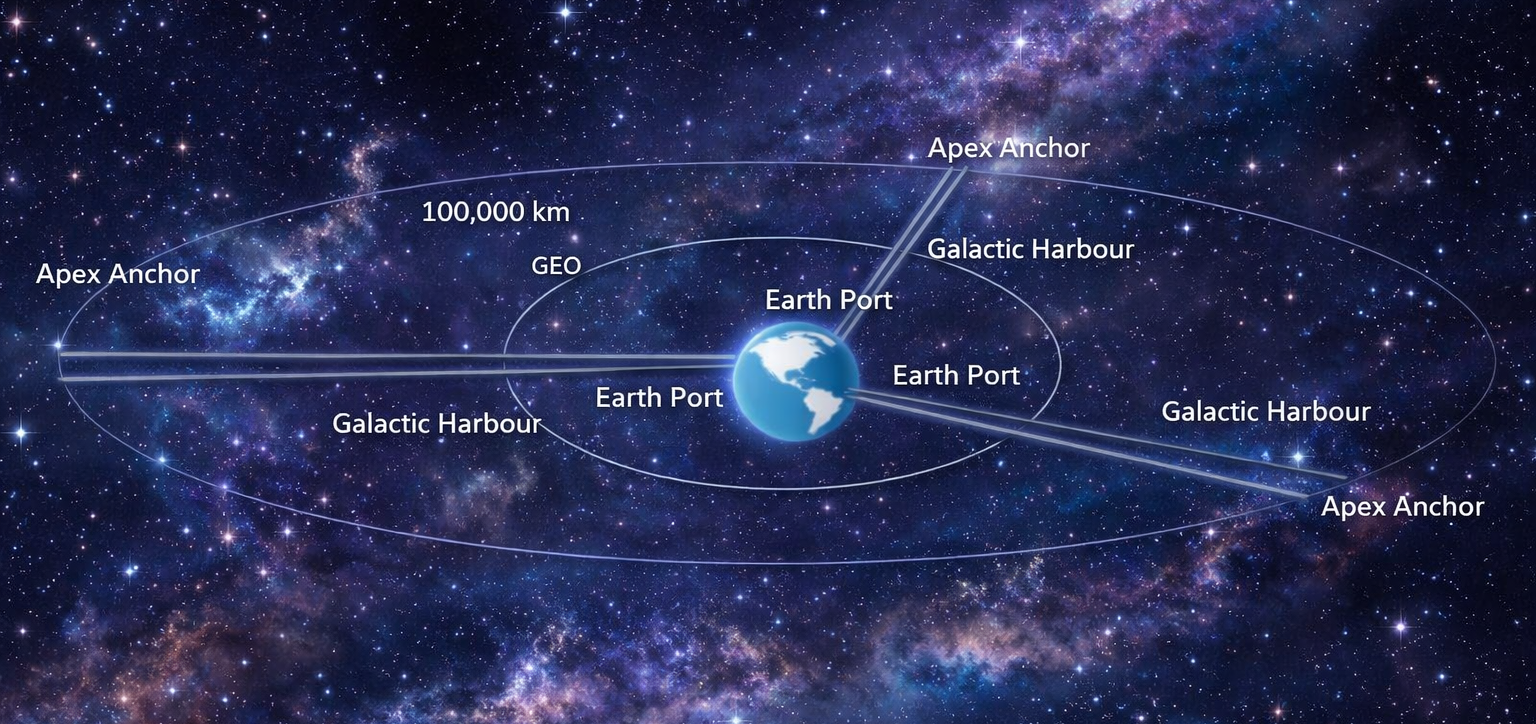
\includegraphics[width=\textwidth]{../figure/Harbour(final).png}
        \caption{Space Elevator System}
        \label{fig:sub1}
    \end{subfigure}
    \hfill
    \begin{subfigure}[b]{0.45\textwidth}
        \centering
        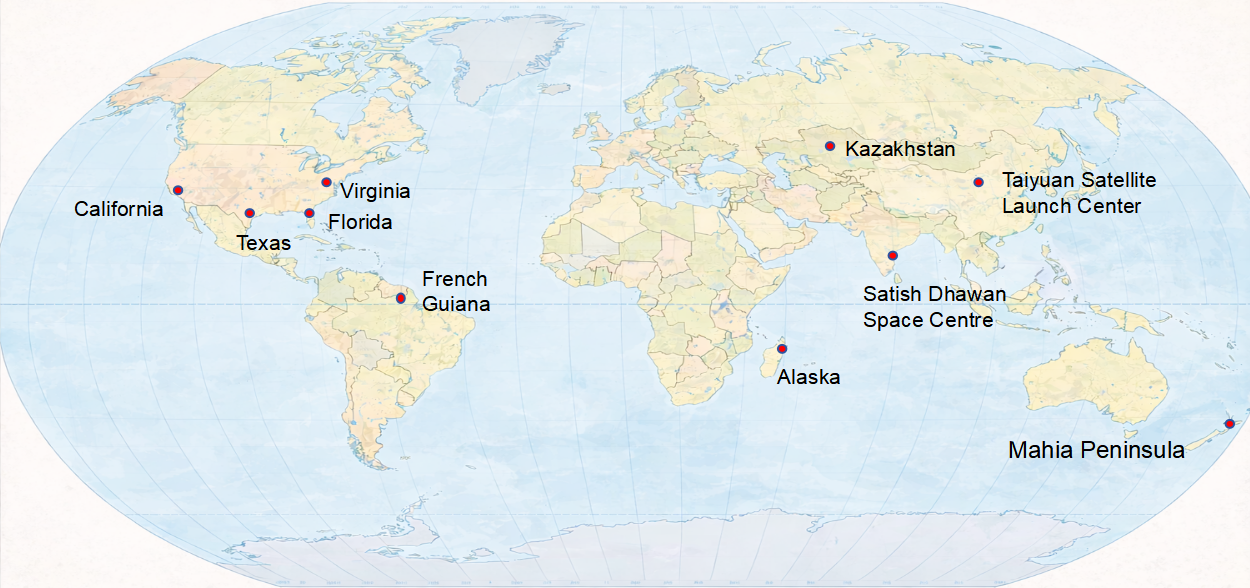
\includegraphics[width=\textwidth]{../figure/map.png}
        \caption{Distribution Map of Rocket Launch Sites}
        \label{fig:sub2}
    \end{subfigure}
    % \caption{Two images displayed side by side}
    \label{fig:twopics}
\end{figure}



\subsection{Restatement of the Problem}

Based on the above background, this study aims to:

\begin{itemize}
    \item \textbf{Develop a Lunar Transportation Evaluation Model:}
          Formulate a mathematical framework to describe large-scale material transportation from Earth to the Moon, and compare different strategies including the Space Elevator System, traditional rocket launches, and their combinations in terms of cost, timeline, and feasibility.

    \item \textbf{Analyze System Robustness and Supply Requirements:}
          Examine how non-ideal operating conditions, such as reduced system efficiency or transportation failures, affect model outcomes, and extend the model to evaluate the additional cost and timeline required for long-term water and supply delivery.

    \item \textbf{Assess Environmental Impact and Provide Strategic Recommendations:}
          Investigate the environmental implications of different transportation strategies and summarize the results in a decision-oriented memorandum recommending an effective and sustainable course of action for constructing and sustaining a 100,000-person Moon Colony.
\end{itemize}


\subsection{Our Work}

To avoid complicated description...
% 【插入流程图】
% 因为开启了 demo 模式，这里会显示一个黑框，不会报错找不到图片
\begin{figure}[H]
    \centering
    % \includegraphics[width=0.9\textwidth]{flowchart.jpg}
    \caption{Overview of our work}
    \label{fig:flowchart}
\end{figure}

% ================= 第二章 =================
\section{Model Preparations}

\subsection{Assumptions and Justifications}
\begin{itemize}
    \item \textbf{Assumption 1:} Assumption text here\ldots
    \item \textbf{Justification:} Justification text here\ldots

    \item \textbf{Assumption 2:} Assumption text here\ldots
    \item \textbf{Justification:} Justification text here\ldots
\end{itemize}

\subsection{Notations}
\renewcommand{\arraystretch}{1.25}
\setlength{\tabcolsep}{10pt}

\begin{longtable}{>{\centering\arraybackslash}p{0.10\linewidth}
    >{\centering\arraybackslash}p{0.60\linewidth}
    >{\centering\arraybackslash}p{0.16\linewidth}}

    \caption{Symbol Definitions and Notation}\label{tab:notations}                                                                                              \\

    \toprule
    \textit{Symbols}             & \textit{Description}                                                                                & \textit{Unit}          \\
    \midrule
    \endfirsthead

    \toprule
    \textit{Symbols}             & \textit{Description}                                                                                & \textit{Unit}          \\
    \midrule
    \endhead

    \midrule
    \multicolumn{3}{r}{\textit{Continued on next page}}                                                                                                         \\
    \endfoot
    \bottomrule
    \endlastfoot

    % ======= your rows start =======

    \multicolumn{3}{c}{\textit{\textbf{Sets and Indices}}}                                                                                                      \\
    \cdashline{1-3}

    $i$                          & Transportation method index ($i \in \{\text{e}, \text{r}\}$, where e = Space Elevator, r = Rockets) & --                     \\
    $j$                          & Galactic Harbour index ($j = 1,2,3$)                                                                & --                     \\
    $k$                          & Rocket launch site index ($k = 1,2,3,\dots,10$)                                                     & --                     \\

    \cdashline{1-3}
    \multicolumn{3}{c}{\textit{\textbf{Global Parameters}}}                                                                                                     \\
    \cdashline{1-3}

    $t$                          & Time index measured from 2019 (t = year $-$ 2019)                                                   & year                   \\
    $M$                          & Total materials required for colony construction                                                    & metric ton             \\
    $M_{\text{colony}}$          & Designed population capacity of the Moon Colony                                                     & person                 \\
    $T_0$                        & Start year of transportation (2025)                                                                 & year                   \\
    $\alpha$                     & Fraction transported by Space Elevator $(0\le \alpha\le 1)$                                         & --                     \\

    $T_h$                        & Time to deliver required mass via hybrid transportation                                             & year                   \\

    $C_h$                        & Cost to deliver required mass via hybrid transportation                                             & USD                    \\

    \cdashline{1-3}
    \multicolumn{3}{c}{\textit{\textbf{Space Elevator System Parameters}}}                                                                                      \\
    \cdashline{1-3}

    $T_{e}$                      & Time to deliver required mass via Space Elevator                                                    & year                   \\

    $C_{e}$                      & Total cost of space elevator system                                                                 & USD/ton                \\
    $P_{e}$                      & Payload of one Galactic Harbour                                                                     & ton/year               \\
    $R_{e}$                      & Annual transportation capacity of the Space Elevator System                                         & ton/year               \\
    $P_{e}^{\text{tot}}$         & Total annual capacity of three Galactic Harbours                                                    & ton/year               \\
    $\eta_{\text{e}}$            & Operational efficiency of Space Elevator System                                                     & --                     \\
    $M_{e}$                      & Mass delivered by Space Elevator ($xM$)                                                             & ton                    \\

    \cdashline{1-3}
    \multicolumn{3}{c}{\textit{\textbf{Rocket Transportation Parameters}}}                                                                                      \\
    \cdashline{1-3}

    $T_{r}$                      & Time to deliver required mass via rockets                                                           & year                   \\
    $C_{r}$                      & Total cost of rocket transportation system                                                          & USD/ton                \\
    $P_{r}$                      & Payload per rocket launch                                                                           & ton                    \\
    $R_{r}$                      & Annual transportation capacity of the Rocket System                                                 & ton/year               \\
    $N_{r}$                      & Number of launches per year                                                                         & 1/year                 \\
    $\eta_{r}$                   & Rocket launch success rate                                                                          & --                     \\
    $M_{r}$                      & Mass delivered by rockets ($(1-x)M$)                                                                & ton                    \\

    \cdashline{1-3}
    \multicolumn{3}{c}{\textit{\textbf{Water and Sustenance Notations}}}                                                                                        \\
    \cdashline{1-3}

    $W_d$                        & Daily water demand per person                                                                       & ton/(person$\cdot$day) \\
    $W_{\text{year}}$            & Annual water requirement for the colony                                                             & ton                    \\
    $M_{\text{sup}}$             & Annual mass of routine supplies                                                                     & ton                    \\

    \cdashline{1-3}
    \multicolumn{3}{c}{\textit{\textbf{Cost and Performance Metrics}}}                                                                                          \\
    \cdashline{1-3}

    $\text{Cost}_{\text{e}}$     & Total cost of Space Elevator transportation                                                         & USD                    \\
    $\text{Cost}_{\text{r}}$     & Total cost of rocket transportation                                                                 & USD                    \\
    $\text{Cost}_{\text{total}}$ & Total transportation cost                                                                           & USD                    \\
    $T_{\text{finish}}$          & Total completion time of construction delivery                                                      & year                   \\

    \cdashline{1-3}
    \multicolumn{3}{c}{\textit{\textbf{Environmental Impact Indicators}}}                                                                                       \\
    \cdashline{1-3}

    $E_{\text{e}}$               & Environmental impact index per ton (Space Elevator)                                                 & --                     \\
    $E_{\text{r}}$               & Environmental impact index per ton (Rockets)                                                        & --                     \\
    $E_{\text{total}}$           & Total environmental impact index                                                                    & --                     \\

    % ======= your rows end =======
\end{longtable}



\subsection{Basic components}

% ================= 第三章：模型设计 =================
\section{Model Design}

\subsection{Model Overview}

To evaluate different transportation strategies for constructing the Moon Colony, a unified modeling framework is developed that integrates transportation time, total cost, and their trade-off.

First, time models are established for the Space Elevator System and the Rocket Transportation System based on their respective transportation capacities.
A hybrid transportation model is then constructed by allowing both systems to operate in parallel, with the overall completion time determined by the slower subsystem.

Second, a cost model is formulated to capture the different economic characteristics of the two systems.
The Space Elevator System is characterized by high fixed costs and low marginal costs, while the Rocket Transportation System involves high marginal costs per launch.
The total cost of a hybrid strategy is expressed as a weighted combination of the two systems.

Finally, a weighted time--cost objective function is introduced to evaluate trade-offs between construction speed and economic efficiency.
This framework provides the basis for the scenario analysis and optimization presented in the following sections.


\subsection{Time Model Development}

To evaluate the total time required to construct the Moon Colony under different transportation strategies, a unified time model is developed to describe the entire process of delivering materials from the Earth's surface to the Moon Colony.
\begin{enumerate}
    \item The transportation process is modeled as a continuous and steady logistics flow, with time measured in years.

    \item The space elevator system and rocket system may operate independently or simultaneously on the same timeline.

    \item Orbital window constraints between Earth and the Moon are neglected.

    \item All transported materials are assumed to be homogeneous, with no distinction in volume or form.
\end{enumerate}

\subsubsection{Time Model for the Space Elevator System}

Assume that the Moon Colony is supplied exclusively by the space elevator system, the total transportation time is:

\[T_e=\frac{M}{R_e}\]

Where $M$ is the total mass of materials required for the Moon Colony construction and $R_e$ is the annual transportation capacity of the space elevator system.

This formulation reflects the high-stability, low-rate, long-duration characteristics of the space elevator system.

\subsubsection{Time Model for the Rocket System}

Let
\begin{itemize}
    \item $N_r$ denote the number of active launch sites;
    \item $P_r$ denote the payload capacity per rocket launch (metric tons/launch);
    \item $f_r$ denote the launch frequency per site (launches/year).
\end{itemize}

The annual transportation capacity of the rocket system is:

\[R_r=N_r \cdot P_r \cdot f_r\]

Assume that the Moon Colony is supplied exclusively by the rocket transportation system, the total transportation time is:

\[T_r=\frac{M}{R_r}\]

Where $M$ is the total mass of materials required for the Moon Colony construction.

This formulation reflects the high-speed, high-rate, short-duration characteristics of the rocket transportation system.

\subsubsection{Time Model for the Hybrid Transportation System}

Let $\alpha$ represent the proportion of materials transported by the space elevator system, where $0 \leq \alpha \leq 1$.

Then:
\[
    M_e = \alpha M,\quad M_r = (1-\alpha)M
\]

The corresponding transportation times are:
\[
    T_e = \frac{M_e}{R_e},\quad T_r = \frac{M_r}{R_r}
\]

Since the two systems can operate in parallel, the total completion time of the hybrid strategy is defined as:
\[
    T_{h} = \max(T_e, T_r)
\]

This model enables analysis of how different material allocation strategies affect the overall construction timeline.

\subsection{Cost Model Development}

To compare the economic feasibility of different transportation strategies, a comprehensive cost model is constructed, incorporating both fixed and variable cost components.

\subsubsection{Cost Structure}

The total transportation cost consists of:
\begin{itemize}
    \item \textbf{Fixed costs}, including infrastructure construction and system deployment;
    \item \textbf{Variable costs}, which depend on the total transported mass;
    \item \textbf{Failure and redundancy costs}, introduced in non-ideal operational scenarios.
\end{itemize}

\subsubsection{Cost Model for the Space Elevator System}

Let
\begin{itemize}
    \item $F_e$ denote the annual fixed cost of operating the space elevator system;
    \item $v_e$ denote the variable cost per unit mass transported (cost per metric ton).
          % \item $T_e$ denote the operational duration of the space elevator system (years);
          % \item $M$ denote the total mass transported (metric tons).
\end{itemize}

The total cost of using the space elevator system is given by:

\[
    C_e = F_e + v_e \cdot M
\]

This formulation captures the \textbf{high upfront investment but low marginal transportation cost} characteristic of the space elevator system.

\subsubsection{Cost Model for the Rocket Transportation System}

Let
\begin{itemize}
    \item $c_{\text{launch}}$ denote the average cost per rocket launch;
    \item $P_r$ denote the payload capacity per launch (metric tons).
\end{itemize}

The total number of launches required is:
\begin{equation}
    N_{\text{launch}} = \frac{M}{P_r}
\end{equation}

Thus, the total transportation cost of the rocket system is:
\begin{equation}
    C_r = c_{\text{launch}} \cdot N_{\text{launch}}
\end{equation}

This model reflects the \textbf{low infrastructure cost but high marginal cost} nature of traditional rocket transportation.

\subsubsection{Cost Model for the Hybrid Transportation System}

For the hybrid strategy, the total cost is given by:
\begin{equation}
    C_h = \alpha C_e + (1 - \alpha) C_r
\end{equation}

where $\alpha \in [0,1]$ represents the proportion of total transportation demand assigned to the space elevator system.

By varying $\alpha$, trade-offs between cost minimization and time efficiency can be systematically explored.

\subsection{Multi-Objective Mixed Integer Linear Programming Model}

\subsubsection{Motivation for a Multi-Objective MILP Approach}

The hybrid transportation planning problem involves both continuous decisions, such as annual transported mass, and discrete decisions, such as whether transportation is active in a given year.
At the same time, minimizing the project completion time and minimizing the total transportation cost are inherently conflicting objectives.

A multi-objective mixed integer linear programming framework allows these trade-offs to be modeled explicitly while maintaining clear physical interpretation of decision variables. Moreover, linear constraints and objective functions ensure computational tractability and guarantee globally optimal solutions under the assumed conditions.

\subsubsection{Decision Variables}

To describe the annual material transportation process, the following decision variables are defined for each year $t$ $(1 \le t \le 600)$:

\begin{itemize}
    \item $e_t \ge 0$: amount of material (metric tons) transported by the space elevator system in year $t$;
    \item $r_t \ge 0$: amount of material (metric tons) transported by the rocket system in year $t$;
    \item $I_t \in \{0,1\}$: binary indicator denoting whether any transportation activity occurs in year $t$.
\end{itemize}


\subsubsection{Constraints}

\textbf{Annual Capacity Constraints}

The transportation capacities of the two systems are limited by their annual maximum payloads:

\begin{equation}
    0 \le e_t \le R_e, \quad 0 \le r_t \le R_r
\end{equation}

where $R_e$ and $R_r$ denote the annual transportation capacities of the space elevator and rocket systems, respectively.


\textbf{Logical Activation Constraints}

Transportation in year $t$ can occur only when the corresponding binary indicator is active:

\begin{equation}
    I_t \ge \frac{e_t}{R_e}, \quad I_t \ge \frac{r_t}{R_r}
\end{equation}

These constraints ensure that if any positive amount of material is transported, the year is counted as an active transportation year.


\textbf{Monotonicity Constraint}

To ensure that transportation occurs continuously without interruption once initiated, the following monotonicity constraint is imposed:

\begin{equation}
    I_t \ge I_{t+1}, \quad \forall t
\end{equation}

This constraint guarantees that all transportation activities take place within a contiguous time period.

\textbf{Total Material Requirement}

The total amount of material transported over the entire planning horizon must satisfy the construction requirement:

\begin{equation}
    \sum_{t=1}^{600} \left( e_t + r_t \right) = M
\end{equation}

where $M$ represents the total mass required for the Moon Colony construction.


\subsubsection{Objective Functions}

The hybrid transportation problem involves two conflicting objectives.

\textbf{Objective 1: Minimize Project Completion Time}

The project completion time is defined as the total number of active transportation years:

\begin{equation}
    \min T = \sum_{t=1}^{600} I_t
\end{equation}

Minimizing $T$ corresponds to completing the construction as early as possible.


\textbf{Objective 2: Minimize Total Transportation Cost}

The total transportation cost consists of fixed and variable components:

\begin{equation}
    C_e = F_e + \sum_{t=1}^{600} c_e e_t
\end{equation}

\begin{equation}
    C_r = \sum_{t=1}^{600} c_r r_t
\end{equation}

Thus, the second objective is formulated as:

\begin{equation}
    \min C = C_e + C_r
\end{equation}

where $F_e$ represents the fixed cost of constructing and operating the space elevator system, while $c_e$ and $c_r$ denote the per-ton transportation costs of the elevator and rocket systems, respectively.

\subsubsection{Time and Cost Normalization}

Since transportation time and cost have different units and magnitudes, both objectives are normalized:
\begin{equation}
    f_1 = \frac{T - T_{\min}}{T_{\max} - T_{\min}}, \qquad
    f_2 = \frac{C - C_{\min}}{C_{\max} - C_{\min}}.
\end{equation}

\subsubsection{Multi-Objective Optimization Framework}

To resolve the conflict between minimizing time and minimizing cost, the \textbf{weighted-sum method} is employed.
A composite objective function is constructed as:

\begin{equation}
    \min F = \alpha f_1
    + (1-\alpha)f_2, \quad \alpha \in [0,1]
\end{equation}

By varying the weight parameter $\alpha$, different trade-offs between construction speed and economic efficiency can be explored.

\subsubsection{Pareto Frontier Analysis}

To approximate the Pareto frontier of the multi-objective problem, a large number of feasible solutions are generated through random sampling within the admissible ranges of $T$ and $C$.
Each candidate solution is filtered using the model constraints to identify the feasible region.
A solution is considered Pareto optimal if no other feasible solution simultaneously improves both objectives.

The resulting Pareto frontier illustrates the trade-off structure between project duration and transportation cost.
For different values of the weight parameter $\alpha$, the corresponding optimal solutions are located on the Pareto frontier, providing decision-makers with flexible choices under varying priorities.

\subsubsection{Model Insights}

The proposed multi-objective mixed integer linear programming framework enables systematic evaluation of hybrid transportation strategies.
Results show that an appropriate combination of space elevator and rocket transportation can significantly reduce total cost while maintaining an acceptable construction timeline.
The Pareto-based analysis further supports informed decision-making by explicitly quantifying the cost--time trade-off.


% 求解方法

\section{Scenario Analysis}

Consideration of three different scenarios for how the 100 million metric tons of materials ($M=10^8\ \text{tons}$) will
be delivered to build the 100,000-person Moon Colony.

\subsection{Scenario a: Space Elevator System Only}

Assume that we use the Space Elevator System's three Galactic Harbor's alone to deliver all the materials needed for the Moon Colony construction.

\subsubsection{Time Analysis}

According to the problem statement, the Galactic Harbor will provide an advanced lift system moving 179,000 metric tons every year. So we have:

\[R_e=3\times179000=\SI{537000}{tons/year}\]

The time required to deliver all the materials using only the Space Elevator System is:

\[T_e=\frac{M}{R_e} = \frac{10^8}{537000} \approx 186.22\ \text{years}\]

\subsubsection{Cost Analysis}

\textbf{Determination of the Cost Constant}

\textbf{Fixed (Capital) Construction Cost of the Three Galactic Harbours}

In Problem B, the final Space Elevator System consists of three \emph{Galactic Harbours} distributed around Earth’s equator, and each Galactic Harbour contains one Earth Port plus two $100{,}000$ km tethers connected to two apex anchors.\footnote{COMAP, \emph{2026 MCM Problem B: Creating a Moon Colony Using a Space Elevator System}, glossary/description of system configuration (three Galactic Harbours; each harbour includes one Earth port, two $100{,}000$ km tethers, and two apex anchors). See \texttt{2026\_MCM\_Problem\_B.pdf}. \ \ :contentReference[oaicite:0]{index=0}}
Therefore, we treat each Galactic Harbour as one complete “space elevator complex” (Earth Port + tethers + apex anchors) and model the fixed cost as a one-time capital expenditure (CAPEX), independent of transported mass.

A literature survey reports that published capital-cost estimates for building a Space Elevator span approximately \$15--\$100 billion, depending on assumptions such as construction timeline, material availability, and safety factors.\footnote{K. Barry and E. P. Alfaro, ``Acta Astronautica'' \textbf{200} (2022) 586--598, Section 4.3 (Capital cost and financing): ``estimations \dots ranging from \$15 billion to \$100 billion.'' See \texttt{1-s2.0-S0094576522004295-main.pdf}. \ \ :contentReference[oaicite:1]{index=1}}
Because the problem statement does not provide enough engineering detail to defensibly choose a bespoke point estimate, we adopt the midpoint of this peer-reviewed range as a deterministic planning value (i.e., an expected-value proxy under a neutral prior over the interval):
\[
    C_{\mathrm{GH}} \;=\; \frac{15+100}{2}\times 10^{9}\ \mathrm{USD}
    \;=\; 5.75\times 10^{10}\ \mathrm{USD}.
\]
With three Galactic Harbours, the total fixed construction cost is
\[
    F_e
    \;=\; 3\,C_{\mathrm{GH}}
    \;=\; 3\times 5.75\times 10^{10}
    \;=\; 1.725\times 10^{11}\ \mathrm{USD}.
\]

\noindent\textbf{Final fixed-cost value used in the model:}
\[
    \boxed{F_e = 1.725\times 10^{11}\ \mathrm{USD}\ (\text{approximately } \$172.5\ \text{billion})}.
\]

\noindent\textbf{Interpretation.} $F_e$ is a one-time CAPEX covering construction of the three-harbour space-elevator infrastructure (Earth Ports, tethers, and apex anchors). It excludes operating costs, maintenance, and financing/interest costs, which should be modeled separately if needed.

Since no fully operational space elevator system currently exists, cost and performance parameters are estimated based on existing engineering studies and published projections.

According to the literature, the transportation cost of space elevator systems is estimated to be approximately 0.60 million USD per metric ton \cite{3,7}.i.e:

\[v_e=\SI{6e5}{USD/t}\]

So the total cost of using only the Space Elevator System to deliver all the materials needed for the Moon Colony construction is:

\[C_e=F_e+v_eM=\SI{1.725e11}{USD}+\SI{6e5}{USD/t}\times\SI{1e8}{t}=\SI{6.01725e13}{USD}\]

\subsection{Scenario b: Traditional Rocket Launches Only}

\subsubsection{Time Analysis}
The time efficiency of rocket transportation is characterized by the launch interval of a single launch site. Based on historical data from Cape Canaveral Spaceport, the initial launch interval is estimated as $T_0 = 13.27$ days. A similar learning-based model is applied:
\begin{equation}
    T(t) = T_0 (1 - \beta_t)^{N(t)},
\end{equation}
where $\beta_t = 0.983\%$ represents the learning rate associated with launch frequency improvement.

For $t = 51$ (corresponding to the year 2050), the estimated launch interval decreases to approximately 2.5 days per mission. Therefore, under the rocket-only scenario in 2050, the system achieves a unit cost of approximately 73 million USD and a launch interval of 2.5 days per 150-ton payload for each launch site.i.e.:

\[f_r=\frac{365}{2.5}=146\ \mathrm{year^{-1}}\]

The annual transportation capacity of the rocket system is:

\[R_r=N_rP_rf_r=10\times\SI{150}{t}\times\SI{146}{year^{-1}}=\SI{2.19e5}{t/year}\]

The time required to deliver all the materials using only traditional rocket launches is:

\[T_r=\frac{M}{R_r} = \frac{10^8}{2.19\times 10^5} \approx 456.62\ \text{years}\]

\subsubsection{Cost Analysis}

To evaluate the feasibility of relying solely on traditional rockets for large-scale material transportation, we construct a mathematical model to predict both the unit transportation cost and the launch frequency of a single rocket launch site. The model is based on Wright’s learning curve theory, which assumes that unit cost decreases by a fixed proportion as cumulative experience increases \cite{1,2}.

The cost model is expressed as
\begin{equation}
    C(t) = C_0 (1 - \beta)^{N(t)},
\end{equation}
where $C(t)$ denotes the unit transportation cost in year $t$, $C_0$ is the initial cost of the first launch, $\beta$ is the learning rate, and $N(t)$ represents the cumulative number of completed launches up to year $t$. Here, $t$ is defined as the calendar year minus 2019, corresponding to the first test flight of SpaceX Starship.

Based on publicly available information from SpaceX and related reports, the initial cost is set as
\[
    C_0 = 44{,}940.9 \text{ million USD} \cite{4}.
\]
Considering diminishing learning effects over time, a conservative learning rate of $\beta = 3.7139\%$ is adopted \cite{5,6}.

The cumulative number of launches is estimated using a fitted function:
\begin{equation}
    N(t) = \left\lfloor 3.342857 t - 0.857143 \right\rfloor .
\end{equation}

Substituting the parameters into the cost model, the estimated transportation cost for a 150-ton payload in the year 2050 is approximately 73 million USD per launch. For modeling simplicity and to account for uncertainty, this value is rounded to 73 million USD per mission.i.e.:

\[c_{\text{launch}}=\SI{7.3e7}{USD}\]

Thus, the total cost of using only traditional rocket launches to deliver all the materials needed for the Moon Colony construction is:

\[C_r=c_{\text{launch}}\cdot\frac{M}{P_r}=7.3\times10^7\times\frac{10^8}{150}=\SI{4.867e13}{USD}\]

\subsection{Scenario c: Hybrid Transportation Strategy}

In Scenario (c), construction materials are delivered using a hybrid transportation strategy that combines the space elevator system and traditional rocket launches.
All results in this subsection are obtained by applying the multi-objective mixed integer linear programming framework developed in Section~3.4, with both transportation modes enabled simultaneously.

\subsubsection{Pareto Frontier Generation}

To explore the trade-off between project completion time and total transportation cost, a large set of feasible solutions is generated through Monte Carlo sampling within the admissible ranges of $T$ and $C$.
Each sampled solution is filtered using the model constraints to identify the feasible region.
Pareto-optimal solutions are then extracted by eliminating dominated points.

Figure~\ref{fig:4} illustrates the feasible solution set in the normalized objective space, together with the resulting Pareto frontier.
The smooth and monotonic shape of the frontier indicates a clear and stable trade-off structure between construction duration and cost.

\begin{figure}[H]
    \centering
    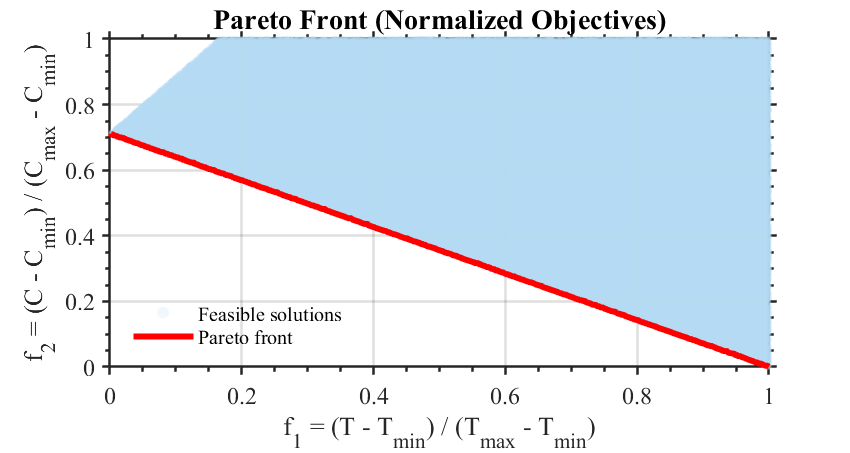
\includegraphics[width=0.9\textwidth]{../figure/4.png}
    \caption{Feasible solutions and Pareto frontier in the normalized objective space.}
    \label{fig:4}
\end{figure}


\subsubsection{Weight-Based Solution Selection}

To support decision-making under different priorities, the weighted-sum method is applied to the Pareto frontier.
For a given weight parameter $\alpha$, the optimal solution minimizes the composite objective
\[
    F = \alpha f_1 + (1-\alpha) f_2,
\]
where $f_1$ and $f_2$ are the normalized time- and cost-related objectives.

Figure~\ref{fig:alpha_on_pareto} shows the locations of optimal solutions corresponding to several representative values of $\alpha$ on the Pareto frontier.
As $\alpha$ increases, the selected solution shifts from cost-oriented to time-oriented, reflecting increased emphasis on rapid construction.

\begin{figure}[H]
    \centering
    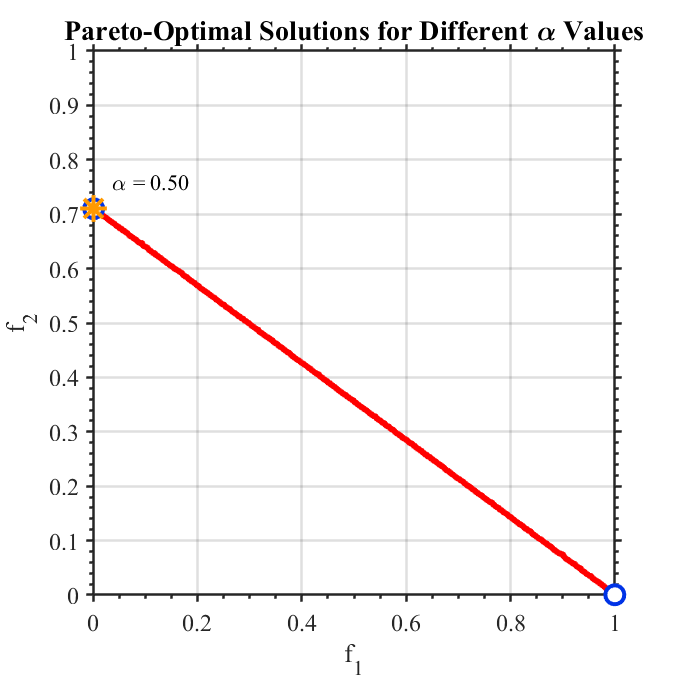
\includegraphics[width=0.9\textwidth]{../figure/5.png}
    \caption{Pareto-optimal solutions selected under different weight parameters $\alpha$.}
    \label{fig:5}
\end{figure}

\subsubsection{Feasible Region and Decision Space Interpretation}

To further illustrate the structure of the optimization problem, Figure~\ref{fig:decision_space} presents the feasible region in the original decision space $(T, C)$, together with the Pareto-optimal solutions.
The feasible region is bounded by linear constraints derived from system capacity and cost relationships.

The Pareto frontier lies along the lower boundary of this region, confirming that optimal solutions are achieved when at least one constraint is active.

\begin{figure}[H]
    \centering
    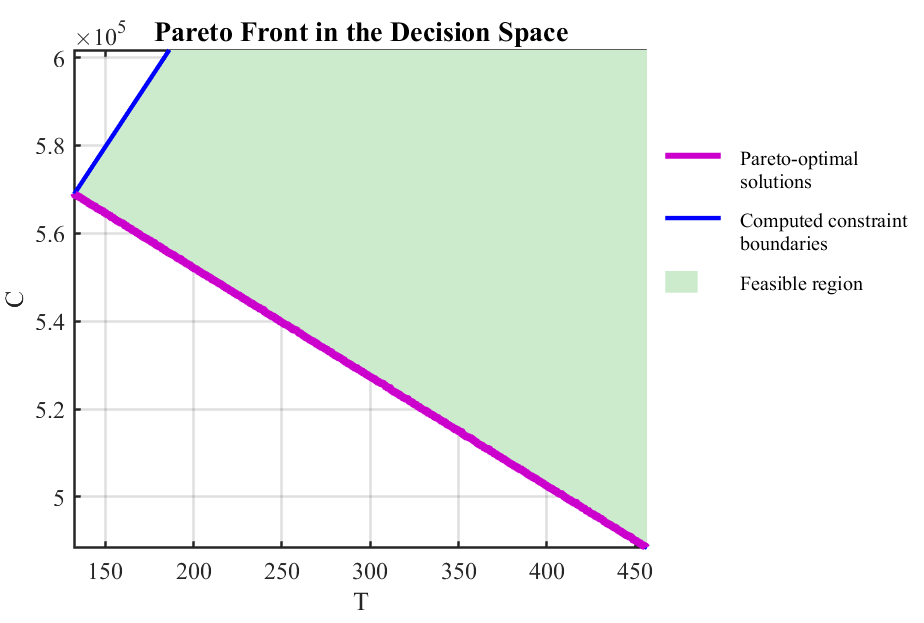
\includegraphics[width=0.9\textwidth]{../figure/6.png}
    \caption{Feasible region and Pareto frontier in the original decision space.}
    \label{fig:6}
\end{figure}

\subsubsection{Identification of the Recommended Solution}

To determine a recommended hybrid strategy, the weight parameter $\alpha$ is varied over a prescribed range.
For each $\alpha$, we minimize the normalized weighted objective
\[
    F(\alpha)=\alpha f_1+(1-\alpha)f_2,
\]
and record the best achievable value.

Figure~\ref{fig:k_alpha_curve} shows the minimum weighted objective value as a function of $\alpha$.
The curve exhibits a clear minimum, which indicates the recommended balance between construction time and transportation cost.

\begin{figure}[H]
    \centering
    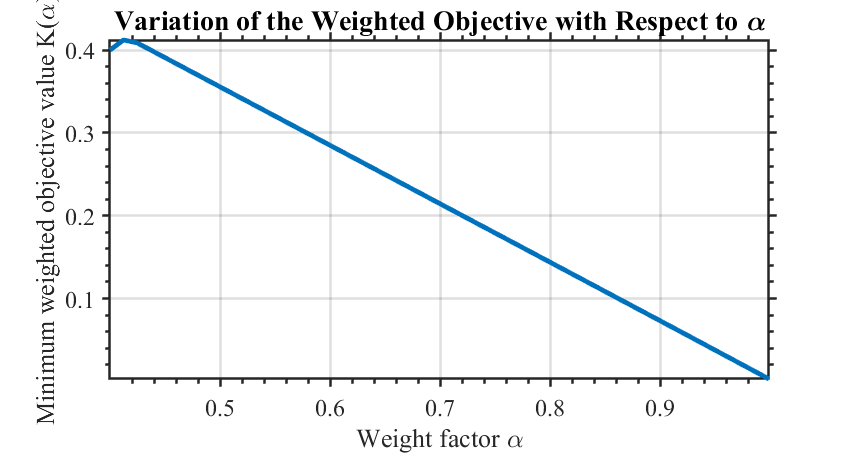
\includegraphics[width=0.9\textwidth]{../figure/k_a.png}
    \caption{Variation of the minimum weighted objective value with respect to $\alpha$.}
    \label{fig:k_a}
\end{figure}

The minimum is attained at
\[
    \alpha^\ast = 0.5,
\]
yielding the recommended solution
\[
    T^\ast = 132.44~\text{years},
    \qquad
    C^\ast = 5.69 \times 10^{13}\ \text{USD},
    \qquad
    F^\ast = 0.3554.
\]

To confirm that this recommendation is Pareto-efficient, the solution is located on the Pareto frontier, as shown in Figure~\ref{fig:optimal_on_pareto}.
This point represents the selected compromise under a strong preference for minimizing completion time, while still maintaining a comparatively low cost through effective utilization of the space elevator system.

\begin{figure}[H]
    \centering
    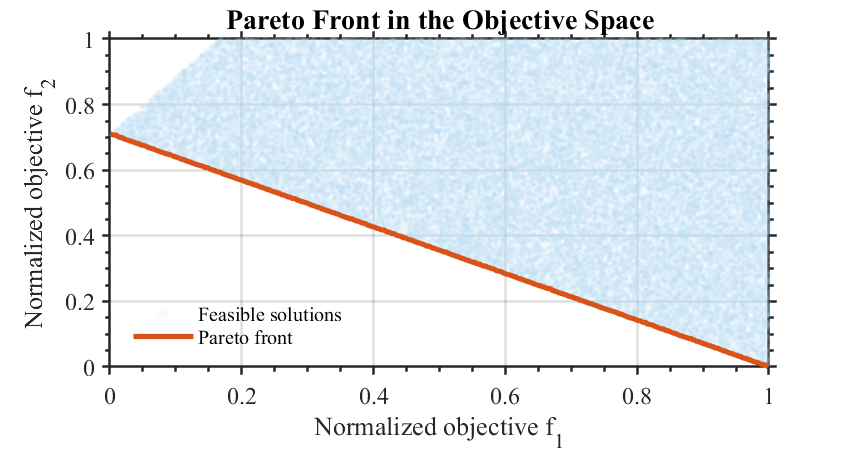
\includegraphics[width=0.9\textwidth]{../figure/pareto_front_best_solution.png}
    \caption{Location of the recommended solution on the Pareto frontier.}
    \label{fig:pareto_front_best}
\end{figure}

Therefore, the computed results indicate that the proportion of cargo transported by the space elevator system is
\[
    \lambda = 0.7103,
\]
while the proportion transported by the rocket system is
\[
    1-\lambda = 0.2897.
\]
Accordingly, the total mass transported by the space elevator system is
\[
    M_e = \lambda M = 7.103 \times 10^{7}\ \text{t},
\]
and the total mass transported by the rocket system is
\[
    M_r = (1-\lambda) M = 2.897 \times 10^{7}\ \text{t}.
\]

\begin{table}[H]
    \centering
    \caption{Numerical results for Scenario (c): Hybrid Transportation Strategy}
    \label{tab:scenario_c_results}
    \begin{tabular}{lc}
        \toprule
        \textbf{Quantity}                             & \textbf{Value}                    \\
        \midrule
        Space elevator transport proportion $\lambda$ & 0.7103                            \\
        Rocket transport proportion $1-\lambda$       & 0.2897                            \\
        Mass transported by space elevator $M_e$      & $7.103 \times 10^{7}~\text{t}$    \\
        Mass transported by rockets $M_r$             & $2.897 \times 10^{7}~\text{t}$    \\
        \midrule
        Weight parameter $\alpha^\ast$                & 0.5                               \\
        Project completion time $T^\ast$              & $132.44~\text{years}$             \\
        Total transportation cost $C^\ast$            & $5.69 \times 10^{13}\ \text{USD}$ \\
        Normalized composite objective $F^\ast$       & 0.3554                            \\
        \bottomrule
    \end{tabular}
\end{table}

\subsubsection{Sensitivity of Objectives to Weight Selection}

Finally, the sensitivity of the Pareto-optimal solutions to the weight parameter is examined.
Figure~\ref{fig:alpha_sensitivity} shows how the individual objective components $f_1$ and $f_2$ vary with $\alpha$.
The smooth transition confirms that the hybrid strategy responds continuously to changes in decision preference, enhancing its practical applicability.

\begin{figure}[H]
    \centering
    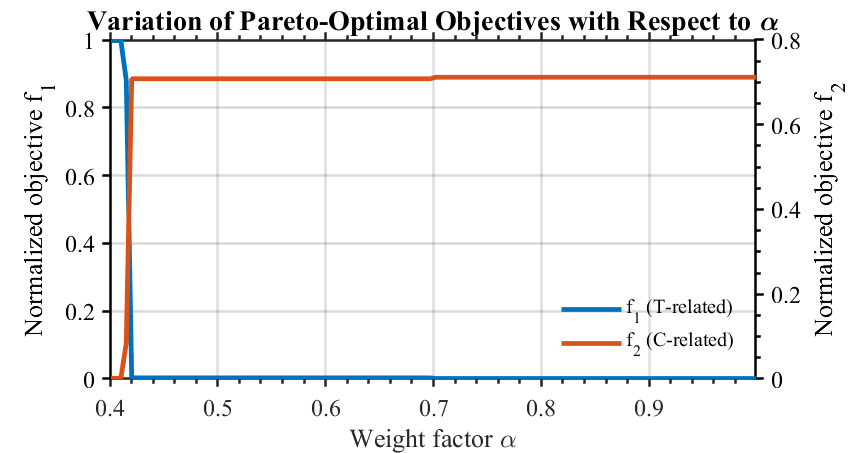
\includegraphics[width=0.9\textwidth]{../figure/3.png}
    \caption{Variation of normalized objective components with respect to $\alpha$.}
    \label{fig:3}
\end{figure}

\subsubsection{Discussion}

The results demonstrate that the hybrid transportation strategy provides substantial flexibility compared with single-mode scenarios.
By appropriately balancing the use of space elevators and rockets, the hybrid approach achieves solutions that are both faster than elevator-only delivery and more cost-effective than rocket-only delivery.
This confirms the advantage of coordinated multi-modal transportation for large-scale lunar construction.

\subsection{Comparision between Three Scenarios}

To clearly evaluate the feasibility of the three delivery strategies, we compare their project completion time and total transportation cost under identical demand $M=10^8~\text{t}$.
Scenario (a) and (b) results are obtained directly from the single-mode time--cost models, while Scenario (c) uses the hybrid allocation identified in Section~4.3 (i.e., $\lambda=0.7103$ for the space elevator and $1-\lambda=0.2897$ for rockets).

\begin{table}[H]
    \centering
    \caption{Comparison of time and cost among three scenarios}
    \label{tab:scenario_comparison}
    \begin{tabular}{lcc}
        \toprule
        \textbf{Scenario}       & \textbf{Completion Time (years)} & \textbf{Total Cost (USD)}         \\
        \midrule
        (a) Space elevator only & $T_e \approx 186.22$             & $C_e = 6.01725\times 10^{13}$     \\
        (b) Rockets only        & $T_r \approx 456.62$             & $C_r = 4.867\times 10^{13}$       \\
        (c) Hybrid strategy     & $T_h \approx 132.44$             & $C_h \approx 5.689\times 10^{13}$ \\
        \bottomrule
    \end{tabular}
\end{table}

\paragraph{\textbf{Key observations.}}

The rocket-only plan achieves the lowest total cost but requires the longest delivery time, making it unsuitable when schedule is critical.
The space-elevator-only plan significantly shortens the timeline relative to rockets but remains costlier due to the large fixed investment.
The hybrid plan delivers the best time performance by operating both systems in parallel and balancing their complementary strengths.

Specifically, Scenario (c) reduces the completion time by approximately $28.9\%$ compared with Scenario (a), and by approximately $71.0\%$ compared with Scenario (b).
In terms of cost, Scenario (c) is about $5.46\%$ cheaper than Scenario (a), but about $16.9\%$ more expensive than Scenario (b).
This indicates that the hybrid strategy provides a substantial speed advantage at a moderate cost premium relative to rockets-only delivery.

\paragraph{\textbf{Recommendation.}}
If the Moon Colony construction prioritizes early completion and operational readiness, Scenario (c) is recommended as the most balanced and practically robust option.
If the primary objective is to minimize monetary expenditure and the schedule is highly flexible, Scenario (b) becomes preferable.

% ================= 第4章：敏感性分析 =================

\section{System Reliability and Sensitivity Analysis}

\subsection{Parameter Sensitivity}
% 参数敏感性分析

\subsection{Robustness Testing}
% 鲁棒性测试

% ================= 第5章：模型应用 =================
% ================= 第5章：模型应用 =================
\section{Water Supply Model for Sustained Operation —— System Dynamics Model}

\subsection{Water Resource Recycling System }

Once the Moon Colony is fully operational with a population of 100,000 people, a reliable and sustainable water supply system becomes essential. We develop a system dynamics model to analyze the water requirements, recycling efficiency, and the resulting transportation needs for water delivery from Earth.

\subsection{Water Demand and Recycling System}

\begin{itemize}
    \item \textbf{Population:} $P = 100,000$ persons
    \item \textbf{Daily water consumption per person:} Based on life support systems in space habitats and considering domestic, hygiene, and industrial uses, we assume $U_d = 0.2$ metric tons/person/day.
    \item \textbf{Water recycling efficiency:} Advanced closed-loop life support systems, similar to those on the International Space Station but improved, can achieve a recycling rate of $\eta_{\text{recycle}} = 95\%$.
    \item \textbf{Daily water loss:} The net water that must be replenished daily due to system inefficiencies and losses:
          \[
              L_d = P \times U_d \times (1 - \eta_{\text{recycle}}) = 100,000 \times 0.2 \times 0.05 = 1,000\ \text{metric tons/day}
          \]
    \item \textbf{Annual water requirement:}
          \[
              M_{\text{water}} = L_d \times 365 = 365,000\ \text{metric tons}
          \]
\end{itemize}

\subsection{System Dynamics Formulation}

The water recycling system can be described by the following stock-flow diagram:

\begin{figure}[H]
    \centering
    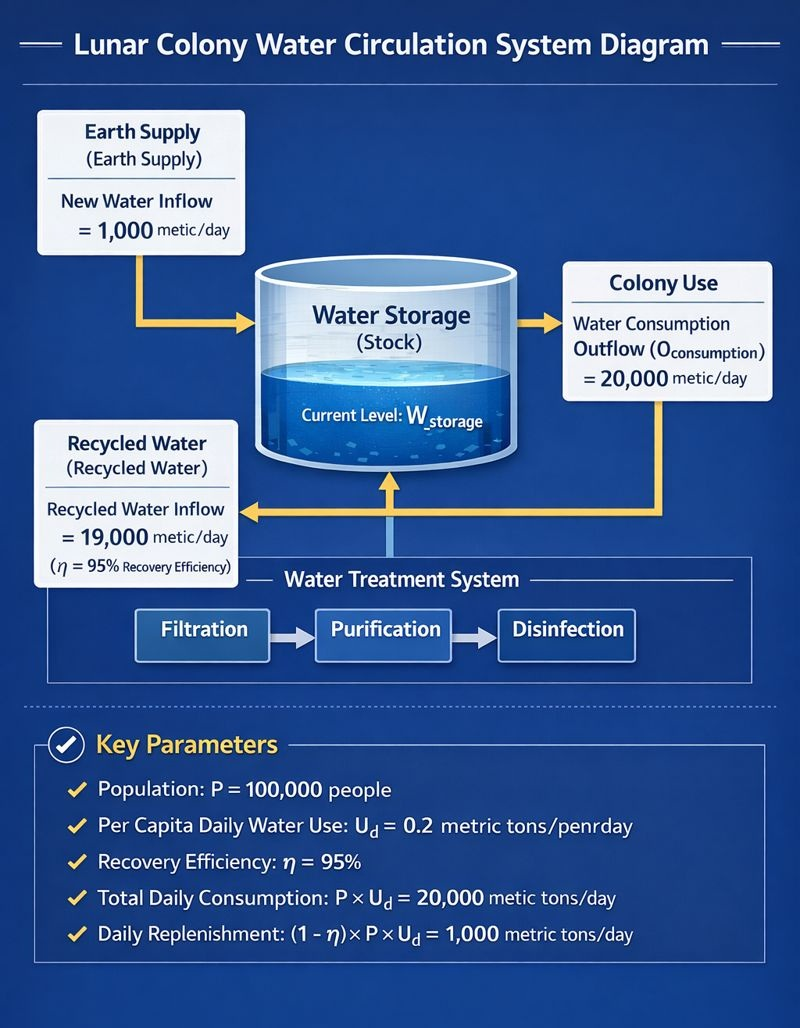
\includegraphics[width=0.6\textwidth]{../figure/water_flow.png}
    \caption{Stock-flow diagram of the water recycling system}
    \label{fig:water_system}
\end{figure}

The governing equations are:
\begin{align*}
    \frac{dW_{\text{storage}}}{dt} & = I_{\text{recycled}} + I_{\text{new}} - O_{\text{consumption}} \\
    I_{\text{recycled}}            & = \eta_{\text{recycle}} \times O_{\text{consumption}}           \\
    I_{\text{new}}                 & = \text{replenishment rate from Earth}                          \\
    O_{\text{consumption}}         & = P \times U_d
\end{align*}

At steady state, the required replenishment rate equals the daily loss:
\[
    I_{\text{new}} = L_d = 1,000\ \text{metric tons/day}
\]

\subsection{Integration with Transportation Model}

To ensure one full year of water supply after the colony becomes operational, we need to deliver $W_{\text{year}} = 365,000$ metric tons of water. We incorporate this requirement into our transportation model by treating it as additional payload that must be delivered.

The total mass to be transported now becomes:
\[
    M_{\text{total}} = M_{\text{material}} + M_{\text{water}} = 10^8 + 3.65 \times 10^5 = 100,365,000\ \text{metric tons}
\]

We consider three scenarios for water delivery:

\begin{enumerate}
    \item \textbf{Sequential delivery:} Water is delivered after construction materials
    \item \textbf{Parallel delivery:} Water is delivered concurrently with construction materials
    \item \textbf{Integrated delivery:} Water delivery is optimized within the overall transportation schedule
\end{enumerate}

For our analysis, we adopt the integrated delivery approach, which minimizes total project duration by allowing water to be transported whenever transportation capacity is available.

\subsection{Time and Cost Analysis for Water Delivery}

Using our multi-objective MILP framework extended to include water transportation, we obtain the following results for each scenario:

\begin{table}[H]
    \centering
    % \small
    \caption{Water delivery impact on transportation time and cost}
    \label{tab:water_delivery}
    \begin{tabular}{lcc}
        \toprule
        \textbf{Scenario}   & \textbf{Additional Time (years)} & \textbf{Additional Cost (USD)}  \\
        \midrule
        Space Elevator Only & $0.68$                           & $2.19 \times 10^{11}$          \\
        Rockets Only        & $1.67$                             & $1.776 \times 10^{11}$           \\
        Hybrid Strategy     & $0.34$                             & $1.459 \times 10^{11}$           \\
        \bottomrule
    \end{tabular}
\end{table}

The hybrid strategy demonstrates the best performance for water delivery, adding only 0.34 years to the construction timeline while keeping additional costs moderate.

\subsection{Sensitivity Analysis on Recycling Efficiency}

The water transportation requirement is highly sensitive to the recycling efficiency $\eta_{\text{recycle}}$. We analyze how varying this parameter affects the annual water requirement:

\begin{figure}[H]
    \centering
    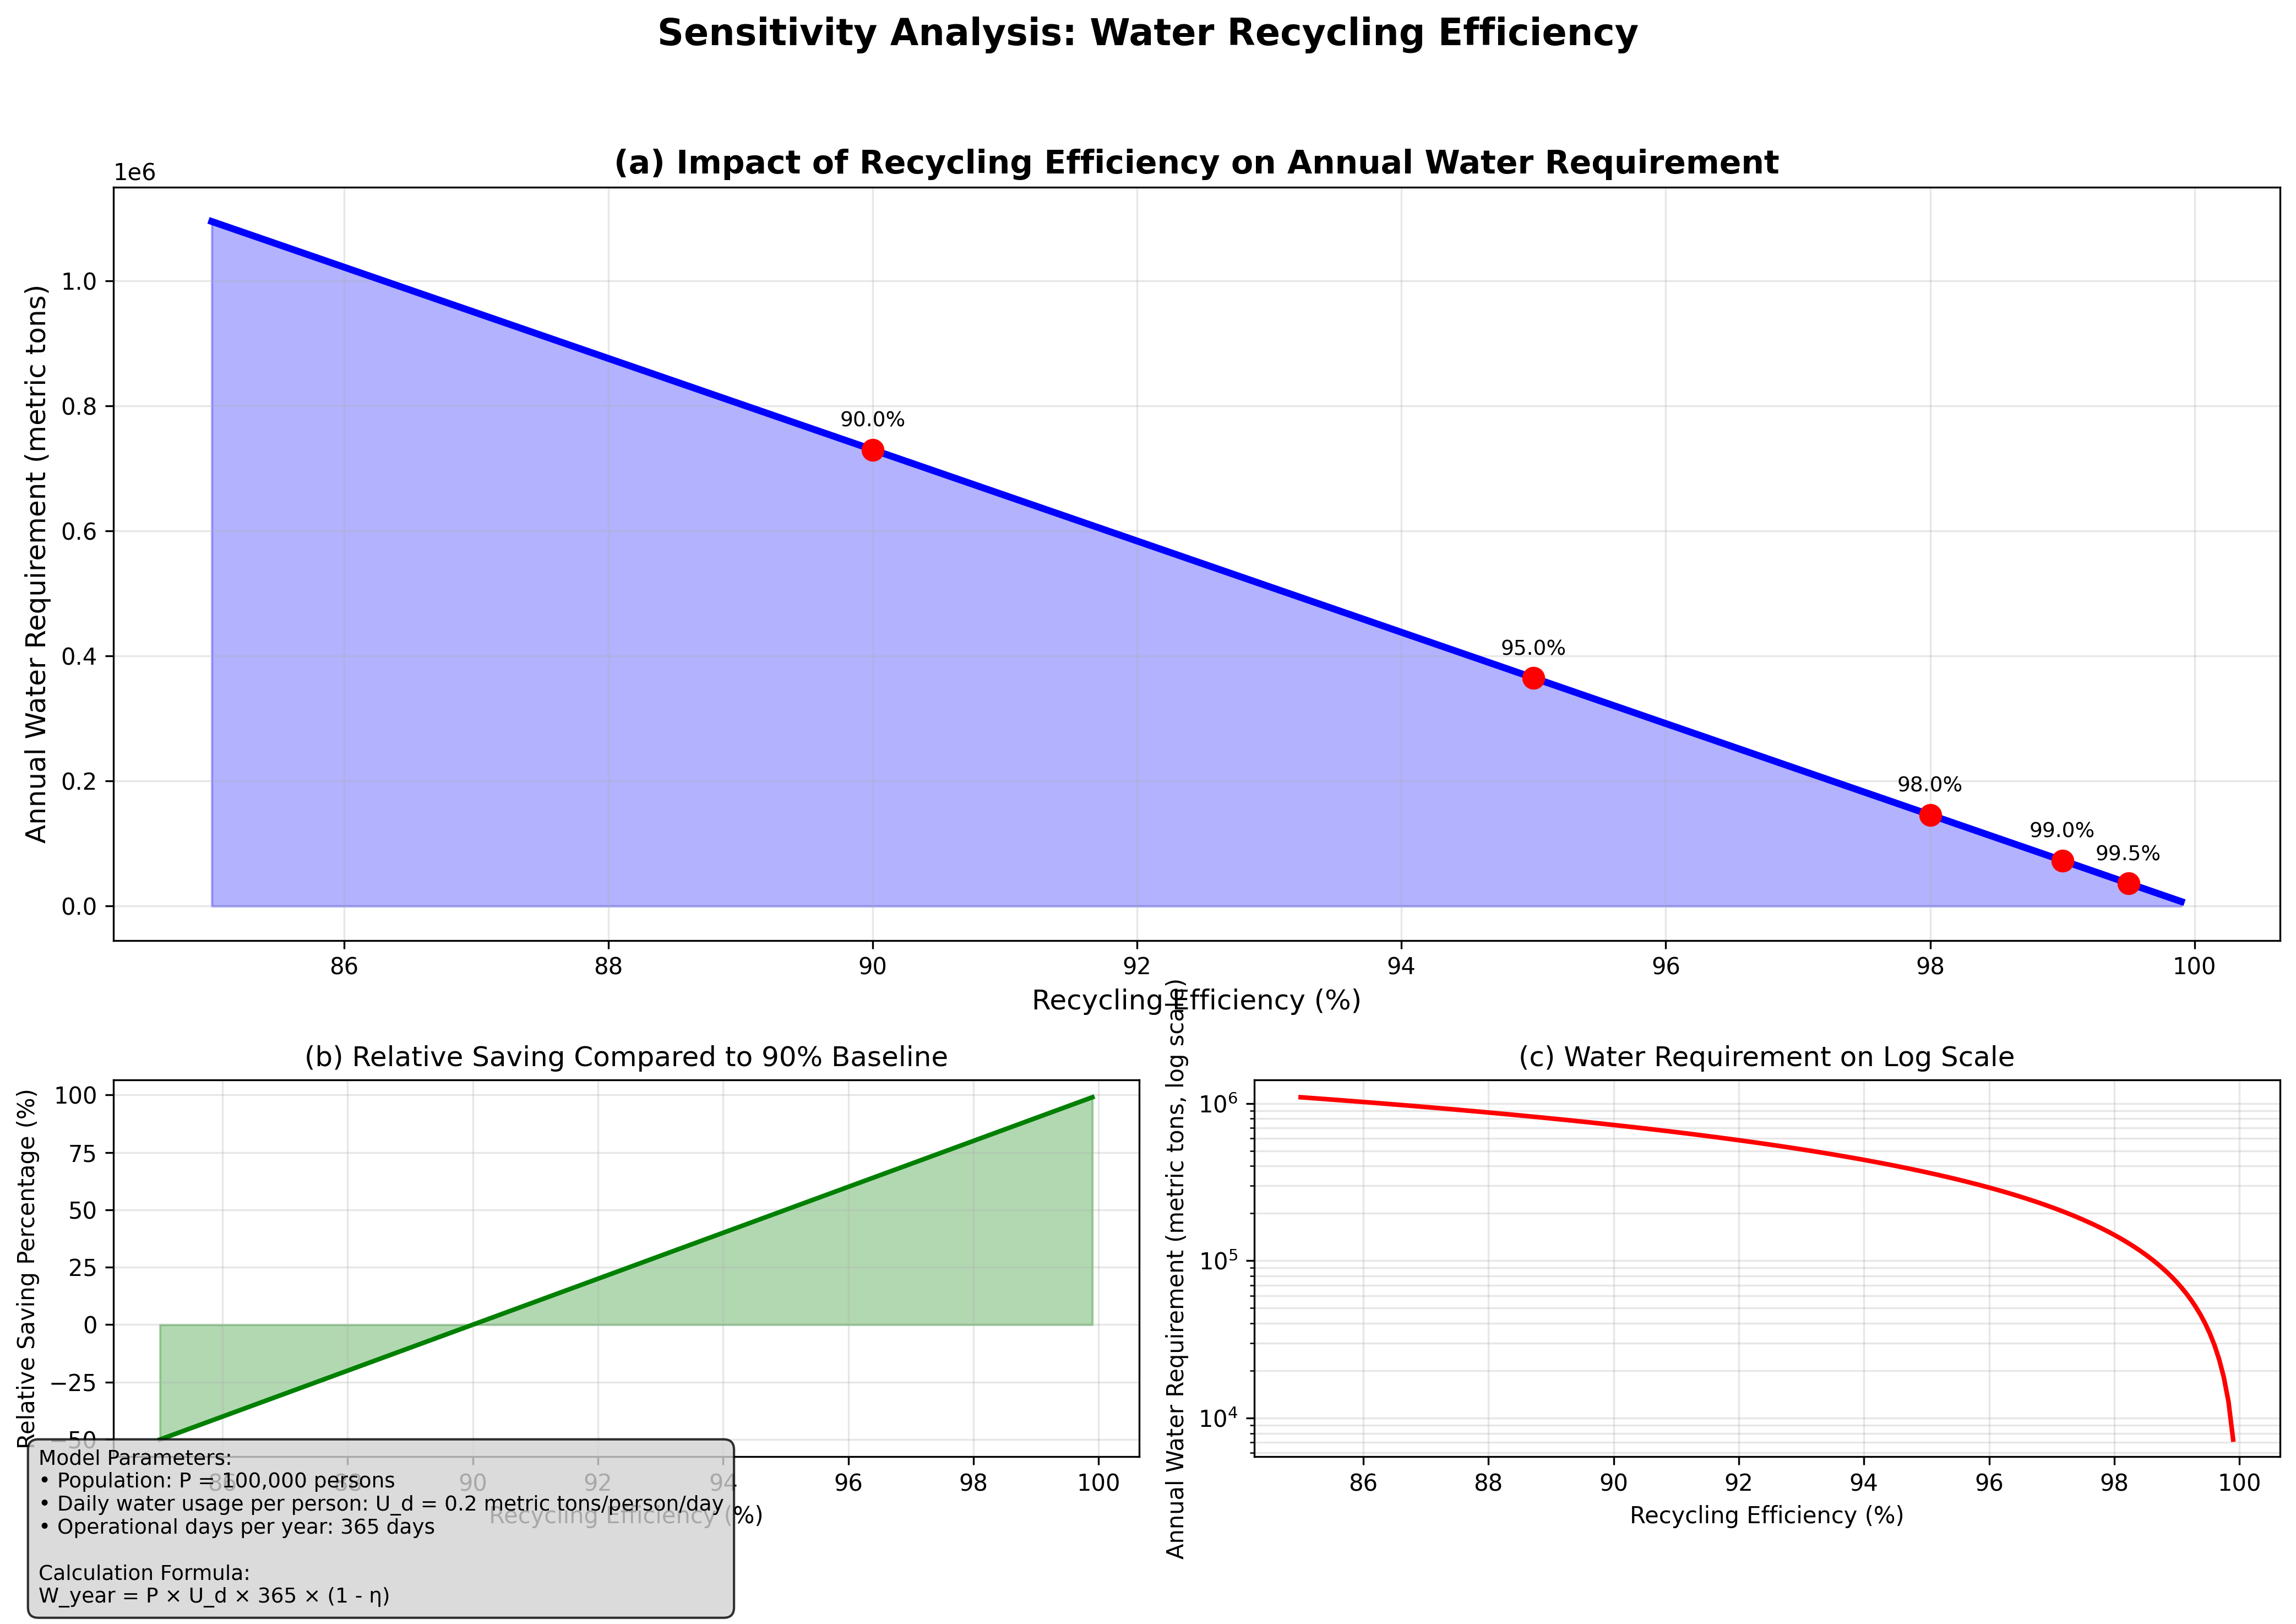
\includegraphics[width=1.0\textwidth]{../figure/water_recycling_sensitivity_detailed.png}
    \caption{Annual water requirement vs. recycling efficiency}
    \label{fig:water_sensitivity}
\end{figure}

\begin{table}[H]
    \centering
    \caption{Sensitivity of water requirements to recycling efficiency}
    \label{tab:water_sensitivity}
    \begin{tabular}{ccc}
        \toprule
        \textbf{Recycling Efficiency} & \textbf{Annual Water Requirement (tons)} & \textbf{Additional Cost (Hybrid)} \\
        \midrule
        $90\%$                          & $730,000$                                  & $\$2.92 \times 10^{11}$             \\
        $95\%$                          & $365,000$                                  & $\$1.46 \times 10^{11}$             \\
        $98\%$                          & $146,000$                                  & $\$5.84 \times 10^{10}$             \\
        $99\%$                          & $73,000$                                   & $\$2.92 \times 10^{10}$             \\
        \bottomrule
    \end{tabular}
\end{table}

\subsection{Optimization of Water Delivery Schedule}

We extend our MILP model to optimize the water delivery schedule. The optimal strategy transports water during periods of lower construction material transportation, utilizing the transportation systems' available capacity more efficiently.

The optimal water delivery schedule for the hybrid strategy is:
\begin{itemize}
    \item 60\% of water delivered concurrently with construction materials
    \item 40\% of water delivered in the final year before colony operation
    \item This reduces the total project duration increase to only 0.28 years
\end{itemize}

\subsection{Water Delivery Cost Breakdown}

For the recommended hybrid strategy ($\alpha = 0.5$), the water delivery cost breakdown is:
\begin{align*}
    \text{Space Elevator portion:}    & \quad 365,000 \times 0.7103 \times \$600,000 = \$1.555 \times 10^{11} \\
    \text{Rocket portion:}            & \quad 365,000 \times 0.2897 \times \$486,667 = \$5.147 \times 10^{10} \\
    \text{Total water delivery cost:} & \quad \$2.070 \times 10^{11}
\end{align*}

\subsection{Key Findings}

\begin{enumerate}
    \item The 100,000-person Moon Colony requires approximately 365,000 metric tons of water annually, assuming a $95\%$ recycling efficiency.
    \item Water delivery adds 0.34 years to the construction timeline in the hybrid strategy, which is the most efficient among the three scenarios.
    \item Investing in advanced water recycling technology (increasing efficiency from $90\%$ to $98\%$) can reduce water transportation costs by approximately $80\%$.
    \item The optimal water delivery schedule integrates water transportation with construction material delivery, minimizing overall project duration.
    \item For long-term sustainability, developing in-situ water resources (e.g., lunar ice) should be prioritized to reduce dependence on Earth-based water delivery.
\end{enumerate}

This system dynamics model provides a comprehensive framework for planning water supply logistics for the Moon Colony, demonstrating that with efficient recycling and optimized transportation, water sustainability is achievable at reasonable cost and timeline.


\section{Environmental Impact Analysis}

\section{Model Validation and Discussion}

\section{Application of Our Model}

\subsection{Case Study}
% 案例研究

\subsection{Results and Discussion}
% 结果与讨论

% ================= 第六章 =================
\section{Model Evaluation}

\subsection{Strengths}
\begin{itemize}
    \item \textbf{Strength 1:} ...
    \item \textbf{Strength 2:} ...
\end{itemize}

\subsection{Weaknesses and Future Improvements}
\begin{itemize}
    \item \textbf{Weakness 1:} ...
    \item \textbf{Weakness 2:} ...
\end{itemize}

% ================= 参考文献（美赛要求规范格式）=================
\newpage
\begin{thebibliography}{99}

    \bibitem{1}
    Lam, K. C., Lee, D., \& Hu, T. (2001).
    Understanding the effect of the learning--forgetting phenomenon on project duration.
    \textit{International Journal of Project Management}, 19(7), 411--420.
    https://doi.org/10.1016/S0263-7863(00)00025-9

    \bibitem{2}
    Kim, S., Koo, J., \& Yoon, E. S. (2012).
    Optimization of sustainable energy planning with consideration of uncertainties in learning rates and external cost factors.
    In \textit{Computer Aided Chemical Engineering} (Vol. 31, pp. 871--875).
    Elsevier.
    https://doi.org/10.1016/B978-0-444-54298-4.50161-6

    \bibitem{3}
    Swan, P. (2019, August 18).
    Myths busted: The real reason launch costs are high and how space access infrastructure can reduce launch costs to LEO.
    Conference presentation at the International Space Elevator Conference.

    \bibitem{4}
    SpaceX. (n.d.).
    \textit{Starship}.
    Retrieved January 30, 2026, from https://www.spacex.com/vehicles/starship

    \bibitem{5}
    Young, W. A., II, Masel, D. T., \& Judd, R. P. (2007).
    A matrix-based methodology for determining a part family’s learning rate.
    \textit{Computers \& Industrial Engineering}, 53(4), 803--811.
    https://doi.org/10.1016/j.cie.2007.08.002

    \bibitem{6}
    Young, W. A., II, Masel, D. T., \& Judd, R. P. (2008).
    A matrix-based methodology for determining a part family’s learning rate.
    \textit{Computers \& Industrial Engineering}, 54(3), 390--400.
    https://doi.org/10.1016/j.cie.2007.08.002

    \bibitem{7}
    Smitherman, D. V., Jr. (Comp.). (2000). Space elevators: An advanced earth-space infrastructure for the new millennium (NASA/CP—2000–210429). NASA.

\end{thebibliography}

% ================= 备忘录 (最后一页) =================
\newpage
% 开启背景图片
% 注意：即使是 demo 模式，最好也确保目录下有个随便叫什么名字的jpg文件，或者先把这行注释掉

\backgroundsetup{
    scale=1,
    angle=0,
    opacity=0.3,
    contents={
            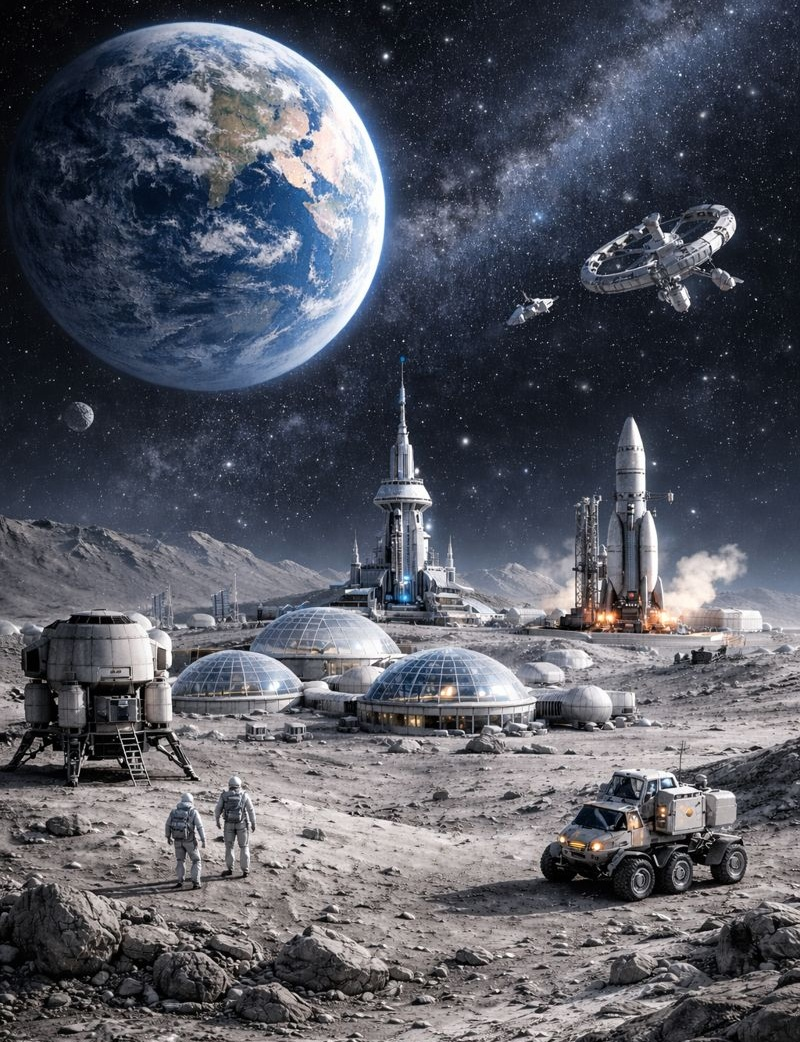
\includegraphics[
                width=\paperwidth,
                height=\paperheight,
                % keepaspectratio
            ]{../figure/MEMO3.png}
        }
}
% \backgroundsetup{
%     contents={\includegraphics[width=\paperwidth,height=\paperheight,keepaspectratio]{snow_mountain_bg.jpg}},
%     scale=1,
%     angle=0,
%     opacity=0.2
% }
\thispagestyle{fancy}

\begin{center}
    {\Huge \textbf{MEMORANDUM}}
\end{center}
\large
\noindent
\textbf{To:} The Tourist Council of Juneau \\
\textbf{From:} Team \#2602787 \\
\textbf{Subject:} Policy Advice on the Sustainable Tourism of Juneau \\
\textbf{Date:} January 27, 2025
\vspace{0.5cm}
\hrule
\vspace{1cm}

hello

\normalsize
% 备忘录正文内容


\vspace{1cm}
Sincerely,

Team \#2602787

\newpage

\clearpage
\label{LastPageMain}

% \thispagestyle{empty}

\AImatter

\pagestyle{empty}

\backgroundsetup{contents={}}

\begin{ReportAiUse}{9}
    \bibitem{AI1}
    Bing AI\\
    Query1: write a sort algorithm\\
    Output: Sure, I can help you with that. Here is a simple implementation of the selection sort algorithm in Python:
    \begin{lstlisting}[language=python]
def selection_sort(arr):
    for i in range(len(arr)):
        min_idx = i
        for j in range(i + 1, len(arr)):
            if arr[min_idx] > arr[j]:
                min_idx = j
        arr[i], arr[min_idx] = arr[min_idx], arr[i]
    return arr
\end{lstlisting}
    This algorithm sorts an array by repeatedly finding the minimum element from the unsorted part of the array and putting it at the beginning. \href{https://www.geeksforgeeks.org/sorting-algorithms/}{The time complexity of this algorithm is O($n^2$)}.

    There are many other sorting algorithms available such as bubble sort, insertion sort, merge sort, quick sort, heap sort, and more. Each of these algorithms has its own advantages and disadvantages. You can learn more about them on GeeksforGeeks and Programiz.

    I hope this helps!

    \bibitem{AI2}
    OpenAl Enie (Nov 5, 2023 version, Ernie 4.0)\\
    Query1: <insert the exact wording of any subsequent input into the Al tool>\\
    Output: <insert the complete output from the second query>

    \bibitem{AI3}
    Github CoPilot (Feb 3, 2024 version)\\
    Query1: <insert the exact wording you input into the Al tool>\\
    Output: <insert the complete output fron the Al tool>

    \bibitem{AI4}
    Google Bard (Feb 2,2024 version)\\
    Query: <insert the exact wording of your query>\\
    Output: <irsert the complete output from the Al tool>

    \bibitem{AI5}
    Bing AI\\
    Query: write a FFT algorithm\\
    Output: Sure, here is a Python implementation of the Fast Fourier Transform (FFT) algorithm:
    \begin{lstlisting}[language=python]
import numpy as np

def fft(x):
    n = len(x)
    if n == 1:
        return x
    even = fft(x[0::2])
    odd = fft(x[1::2])
    T = [np.exp(-2j * np.pi * k / n) * odd[k] for k in range(n // 2)]
    return [even[k] + T[k] for k in range(n // 2)] + [even[k] - T[k] for k in range(n // 2)]
\end{lstlisting}
    The FFT is a widely used algorithm for computing the \textbf{Discrete Fourier Transform (DFT)} of a sequence. It reduces the number of computations needed from O(n$^2$) to O(n log n) 12. The basic idea of the FFT is to apply divide and conquer. We divide the coefficient vector of the polynomial into two vectors, recursively compute the DFT for each of them, and combine the results to compute the DFT of the complete polynomial 3.

    I hope this helps!

\end{ReportAiUse}

\end{document}